% $Id: evaluation.tex 1784 2012-04-27 23:29:31Z nicolas.cardozo $
% !TEX root = main.tex

\chapter{Evaluation}
\label{cha:evaluation}

To evaluate and validate \ac{Flik} as a framework to support the development 
of \ac{RL} programs, and in consequence to help increase their quality, 
an initial empirical evaluation was done. The evaluation consists of three different test scenarios 
from real-world problems that arise in the development of \ac{RL} programs, and the evaluation aimed

The purpose of the evaluation is to observe three scenarios: gridwrold, rooms and cars that cover from 
the creation of an \ac{RL} program from scratch to the process of optimizing 
learning parameters, aiming to determine the specific values to start with 
to achieve the most optimal convergence for the program. In each of the programs a bug 
is added ensuring strange application behavior, but ensuring the application to run, 
therefore, the expected output does not match the real output of the programs. The intention of 
the evaluation scenarios is to if \ac{Flik} can actually improve the performance and developement of \ac{RL}
programs.

The empirical evaluation is performed with a group of students from the \ac{RL} course at Universidad de 
los Andes. We attached the evaluation guide given to the students in \fref{sec:eval-guide}, in which 
is described the purpose of the tool, the description of the activity with the steps on how to run and 
use the tool, a small documentation of the tool, and an small example.

\section{Exercise 1: GridWorld}
\label{sec:grid-eval}

The gridworld environment, used in the evaluation, consists of a $n\times n$ ($10\times 10$ in our example) rectangular 
board/grid, in which each tile $(i,j)$ represents a specific state of the board. Tiles in the board may be 
walls, which agents cannot cross. Additionally, there are special exit 
tiles that give a positive or negative reward to agents, as shown in \fref{fig:gridworld}. All tile types 
are unknown to the agent that moves from a given starting point in the board, searching for the goal 
state (\ie exit states with positive reward of $1$). The agent moves from state to state, avoiding 
obstacles and incorrect exit states (which give a reward of $-1$ when used to exit). 

\begin{figure}[h]
  \centering
  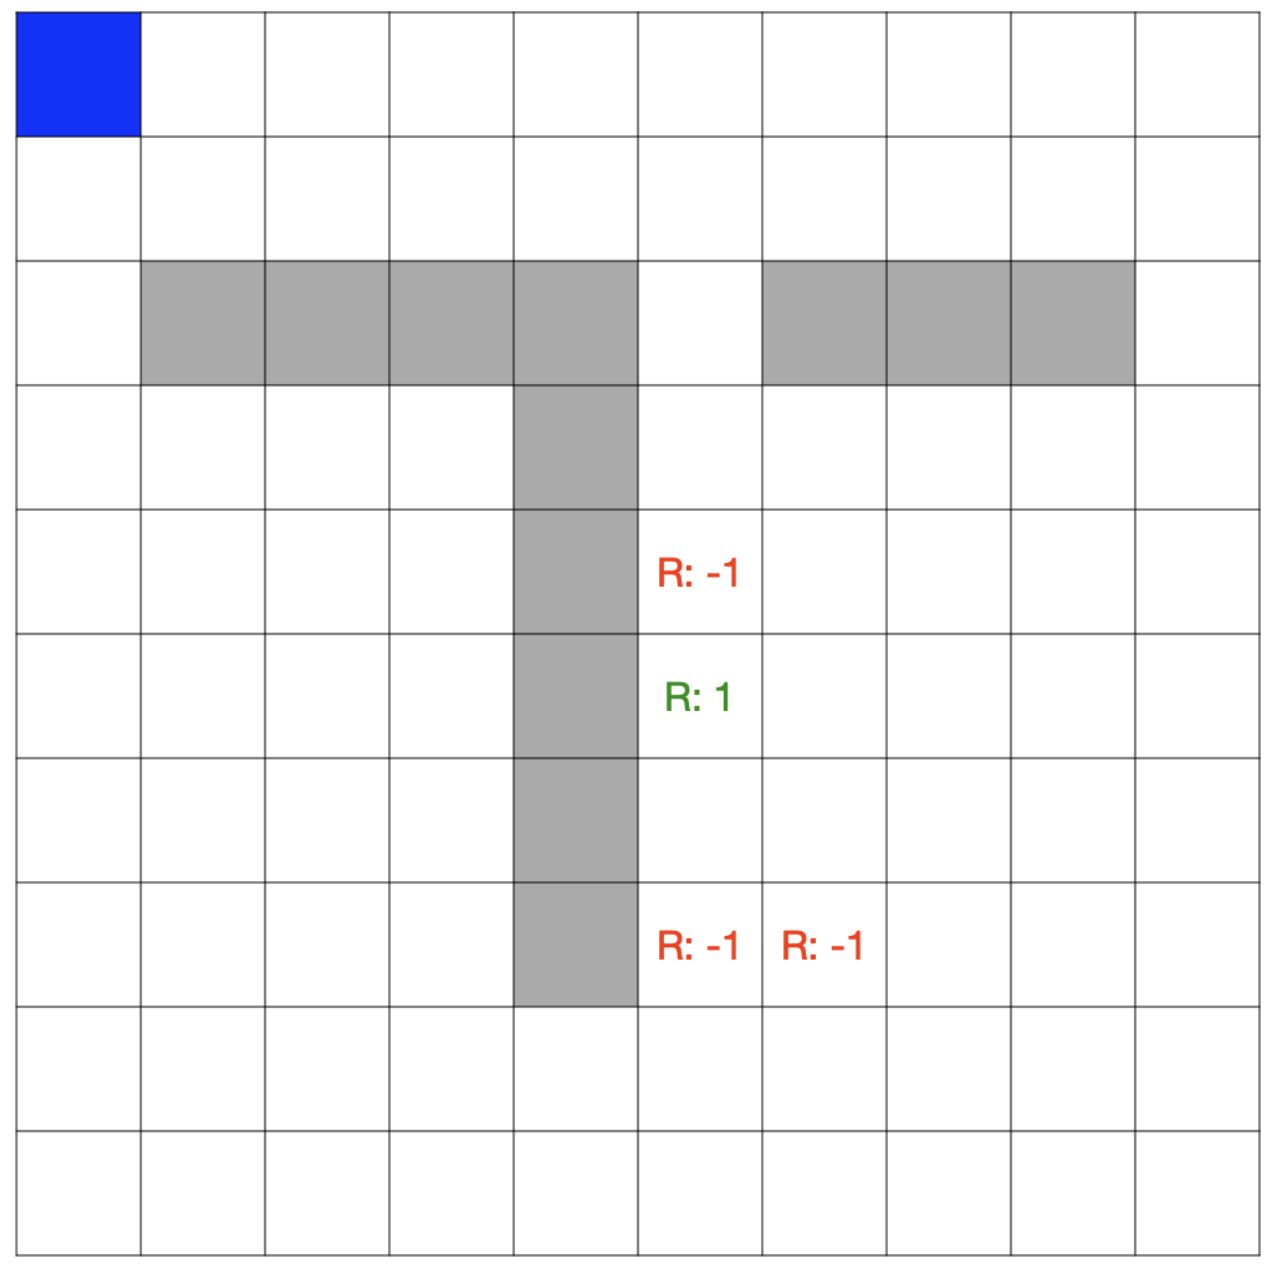
\includegraphics[width=0.5\columnwidth]{figures/gridworld.png}
  \caption{10x10 gridworld environment example}
  \label{fig:gridworld}
\end{figure}

This example introduces a bug for the $\epsilon$ parameter, presenting an error in the probability which
defines which action is taken next. This will introduce a wrong behavior for the \ac{RL} 
agent because $\epsilon$ will be so small that only in the first iteration the action will be taken randomly 
and in the follow interations the probability will be so small to take another action that the agent will not explore
other action policies. This is very bad specially for training purposes as we are supposed to have a very big 
probability to choose other actions and explore the grid. The idea in this task is that the developers
use \ac{Flik} to navigate through the code and find out why is the agent not learning properly. And eventually,
developers should come out with the solution of increasing the value of $\epsilon$. 

\section{Exercise 2: Rooms}
\label{sec:rooms-eval}

The four rooms maze environment consists of a $13\times 13$ board/grid divided in $4$ sections 
(\ie rooms), with walls between them, and a door opening to go from one room to another, as shown 
in \fref{fig:rooms}. The agent's objective in this environment is to exit through the upper-left room 
(the green square) in the fewest possible steps. Reaching the exit state gives a reward of $1$, and no 
other action give a reward to the agent. In each episode the agent starts from any valid position in the 
grid, \eg the yellow square in the bottom-right room in the figure. 

\begin{figure}[h]
  \centering
  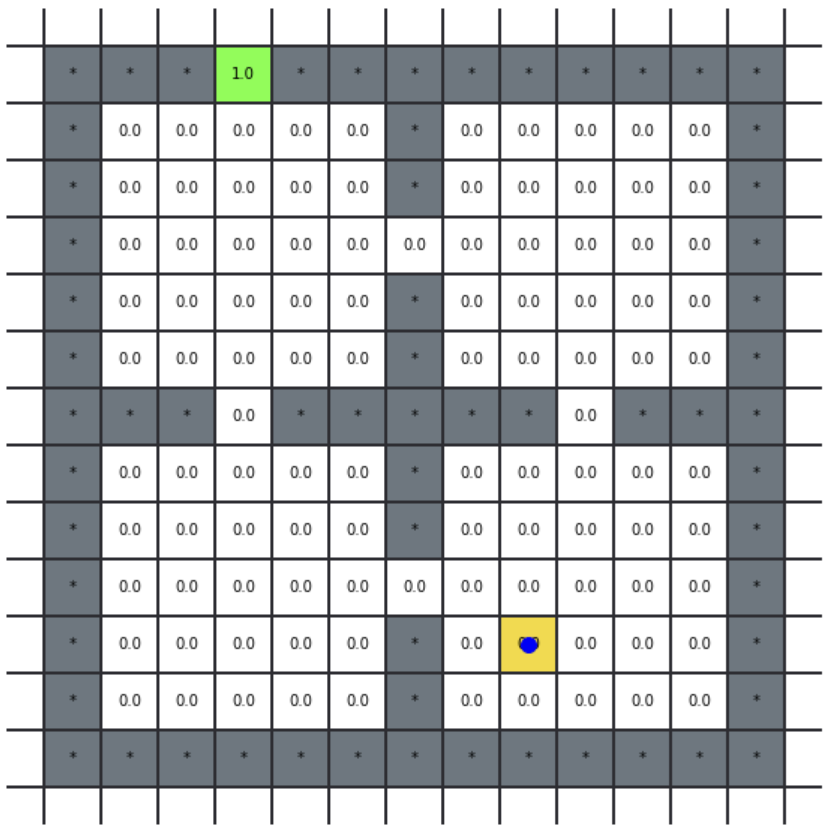
\includegraphics[width=0.5\columnwidth]{figures/rooms.png}
  \caption{Rooms environment example with associated rewards in each state}
  \label{fig:rooms}
\end{figure}

In this example, we introduced a bug in the learning rate $\alpha$, on the Q-learning equation 
so the original values for the learning rate alpha are exchanged like:

Original equation:
$
Q(s, a) \leftarrow (1-\alpha) Q(s, a) + \alpha \left( r + \gamma \max_{a'} Q(s', a') \right)
$

Wrong equation to debug:
$
Q(s, a) \leftarrow  \alpha Q(s, a) + (1-\alpha) \left( r + \gamma \max_{a'} Q(s', a') \right)
$

In the original equation,  $(1-\alpha) Q(s, a)$ is the current value and $\gamma \max_{a'} Q(s', a')$ 
the maximum reward that can be obtained from state $s'$. This means that if the learning rate is very 
small the current value will keep almost the same, turning a little bit towadrs the reward and the 
maximum value given the action, this will make that the agent learn short steps towards the 
optimal policy. Now, in Q-learning, the learning rate $\alpha$ defines how much the old estimate $Q(s,a)$ 
is revised based on the new information. It ensures that over time, the algorithm balances past 
knowledge with current learning, gradually incorporating new information while retaining important 
aspects of previous learning. Changing the equation in this way will disrupt this balance. Specifically,
$(1-\alpha)$ scales the difference between the new estimate and the old estimate. This makes the new 
information less influential as $\alpha$ gets larger, while the old value gets rescaled by $\alpha$, 
which does not align with the expected behavior of a Q-learning update. The idea in this task is that 
the developers use \ac{Flik} to navigate through the code and find out the reason for the agent is not 
learning properly, and why is this happening; comming out to a solution adjusting the value to update the 
Q-Learning equation.

\section{Exercise 3: Driving Assistan}
\label{sec:cars-eval}
In this example the agent must learn to drive, on the correct lane, at the allowed speed, taking over slow 
traffic, and not crashing. The possible actions for the agent are: straight, slow\_down, speed\_up, 
steer\_left, steer\_right. The following is the visual interface of this environment.

\begin{figure}[h]
    \centering
    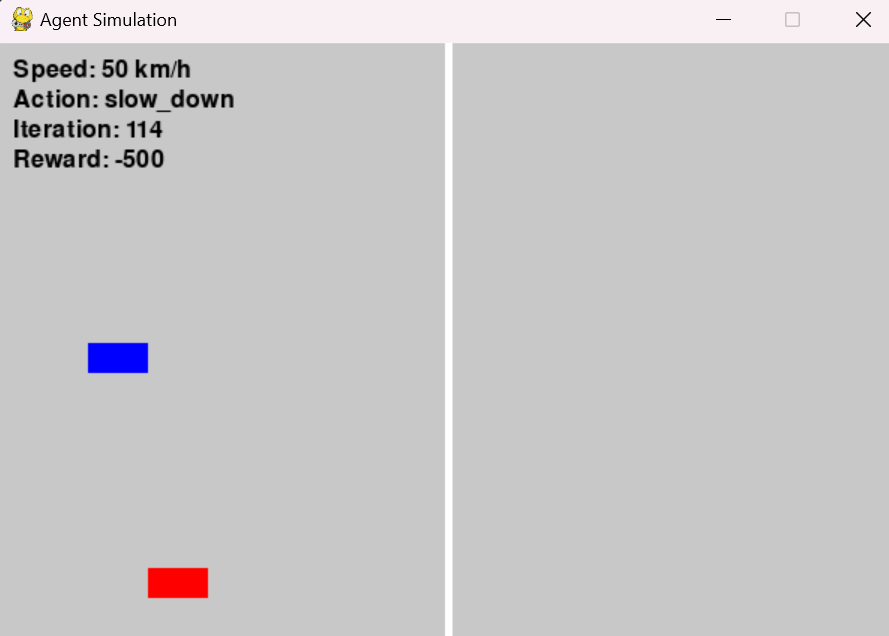
\includegraphics[width=0.5\textwidth]{figures/cars_example.png}
    \caption{Cars code example}
    \label{fig:cars-code-example}
\end{figure}

This is the largest task for the developers to analyze with \ac{Flik} and see why the agent was not learning
correctly, with respect to the expected. The bug introduced in this application is in the reward function,
not motivating the agent to drive at the speed limit. The policy learned by the agent emerges as stopping 
or go very slow, which is not the expected behavior. Through exploration using \ac{Flik}, developers are 
expected to observe the behavior of the reward and update it so that the agent can learn to drive appropriately.
as expected.

% Add way of evaluation, explanation about the survey, questions.
\section{Evaluation setup}
\label{sec:evaluation}
We invited 27 graduate students from Universidad de los Andes that attend the empirical evaluation session. 
The students had the previous three tasks to complete, and it was going according to time. The first 
15 minutes were explanation of the tool and an example of the usage (shown in \fref{sec:eval-guide}).
Then the students had 15 minutes to finish the first task, 15 minutes to finish the second task, and 
20 minutes to finish the third task. The students were asked to fill a survey in a google 
form, which was divided in three main sections: general knowledge questions, task questions, and feedback.
The general knowledge questions were about the experience of the student using Python, debuggers and 
terminal. The task questions were about the bug encountered in each of the tasks, and the solution 
to the problem. The feedback for the debugger usability was about the use of the debugger for the tasks, 
and additional feedback they could provide. The survey was anonymized, the questions were inspired by the 
back in time debugger for JavaScript\cite{delorean23}, and the responses are available 
at \url{https://uniandes-my.sharepoint.com/:x:/g/personal/la_rodriguez_uniandes_edu_co/ESDy89Q-PgVBpYHEZ_CDh_IBhjhS35VFqNrlEjVw_ShY1w?e=lm319K}.
The survey had 23 multiple choice questions in which 5 meant completely agreed, and 1 meant completely disagreed.
One of the questions was a yes or no answer, to identify if the students wanted to use the tool in the future,
or for the class of \ac{RL}. And 10 answers were open questions, to dive deeper into feedback for the tool,
and the tasks' complexity.

Finally, there are two examples of the tool being used. In the first 
example, the tool is used to debug a simple program, this was used to introduced to the students 
the simple commands they could use like stepping (forward and backwards), modifying, or inspecting 
variables. In the second example, the tool is used to debug a \ac{RL} program, specially 
the gridworld example. The link to find this videos is: \url{https://drive.google.com/drive/folders/1dIh9PpnAo23oIuxgzdSGKO39uMChGWKm?usp=sharing} 



\endinput

